\documentclass[a1paper,portrait,fontscale=0.43]{baposter}

\columnsep=70pt % This is the amount of white space between the columns in the poster
\columnseprule=3pt % This is the thickness of the black line between the columns in the poster

\usepackage{wrapfig}
\usepackage{lmodern}

\usepackage[utf8]{inputenc} %unicode support
\usepackage[T1]{fontenc}


\selectcolormodel{cmyk}

\graphicspath{{figures/}} % Directory in which figures are stored


\newcommand{\compresslist}{%
\setlength{\itemsep}{0pt}%
\setlength{\parskip}{1pt}%
\setlength{\parsep}{0pt}%
}

\newenvironment{boenumerate}
  {\begin{enumerate}\renewcommand\labelenumi{\textbf\theenumi.}}
  {\end{enumerate}}



\begin{document}


\definecolor{darkgreen}{cmyk}{0,0.90,0.74,0.28}
\definecolor{lightgreen}{cmyk}{0,0.90,0.74,0.28}

\begin{poster}
{
grid=false,
headerborder=open, % Adds a border around the header of content boxes
colspacing=1em, % Column spacing
bgColorOne=white, % Background color for the gradient on the left side of the poster
bgColorTwo=white, % Background color for the gradient on the right side of the poster
borderColor=darkgreen, % Border color
headerColorOne=lightgreen, % Background color for the header in the content boxes (left side)
headerColorTwo=lightgreen, % Background color for the header in the content boxes (right side)
headerFontColor=white, % Text color for the header text in the content boxes
boxColorOne=white, % Background color of the content boxes
textborder=rounded, %rectangle, % Format of the border around content boxes, can be: none, bars, coils, triangles, rectangle, rounded, roundedsmall, roundedright or faded
eyecatcher=false, % Set to false for ignoring the left logo in the title and move the title left
headerheight=0.11\textheight, % Height of the header
headershape=rounded, % Specify the rounded corner in the content box headers, can be: rectangle, small-rounded, roundedright, roundedleft or rounded
headershade=plain,
headerfont=\Large\textsf, % Large, bold and sans serif font in the headers of content boxes
%textfont={\setlength{\parindent}{1.5em}}, % Uncomment for paragraph indentation
linewidth=2pt % Width of the border lines around content boxes
}
{}
%
%----------------------------------------------------------------------------------------
%	TITLE AND AUTHOR NAME
%----------------------------------------------------------------------------------------
%
{
\textsf %Sans Serif
{Machine Learning Techniques for the Determination and Prediction of Online Gambling Addiction
}
} % Poster title
% {\vspace{1em} Marta Stepniewska, Pawel Siedlecki\\ % Author names
% {\small \vspace{0.7em} Department of Bioinformatics, Institute of Biochemistry and Biophysics, PAS, Warsaw, Pawinskiego 5a}} % Author email addresses
{\sf\vspace{0.5em}\\
David Farrugia* and Dr Lalit Garg
\vspace{0.1em}\\
\small{Faculty of Information and Communication Technology, University of Malta
\vspace{0.2em}\\
david.farrugia.15@um.edu.mt}
}
{
\includegraphics[width=0.1\textwidth]{logo}} % University/lab logo


\headerbox{1. Introduction}{name=introduction,column=0,row=0, span=3}{
Gambling is a form of entertainment where numerous players frequently fall in love with the thrill and the roller-coaster of emotions that the whole playing experience entails. However, gambling may become the root of the destruction of their lives due to falling victims of addiction, which often wills its victims into experiencing other mental and physical issues, such as depression, distress, and anxiety symptoms. This impulse-control habit leaves the victims it haunts lacking self-control and rather effortless in trying to reduce or stop such behaviour \cite{noauthor_gambling_nodate}. This habit is becoming more and more of a problem, in fact, in the year 2013 alone, statistics \cite{noauthor_global_2011} show that the online gambling market generated a revenue of 6.1 billion. Statisticians and researchers predict an increase of 10.1\% in 2018 \cite{noauthor_global_2011}. Without the proper and necessary precautions and measures, the latter results in the victim continually seeking to engage in this unhealthy behaviour; hence, meaning that the problem only gets bigger and bigger \cite{goodman_addiction:_1990}. Thus, this research aims to contribute to this problem by evaluating and proposing some novel and existing machine learning techniques to help predict such pathological behaviour with the effort of controlling the gambling environment.
}


\headerbox{2. Materials and Method}{name=model,column=0,below=introduction,span=1}{

Python was the programming language utilised for all data and model analysis, and application development purposes. Some third-party libraries used in this experiment were: PyQt5, numpy, pandas, pickle, scikit-learn, xgboost, lightgbm, rgf, elm, keras and tensorflow.\\

All data was cleaned accordingly prior evaluation. Furthermore, by using cross-validation techniques, the data was split up into training and testing sets. The training of all models by fitting the training sets (all data split into partitions by cross-validation) was then followed by fitting the testing features to obtain a prediction set. In turn, by utilising these predictions for evaluation, some scoring metrics resulted for comparison.
\begin{center}
    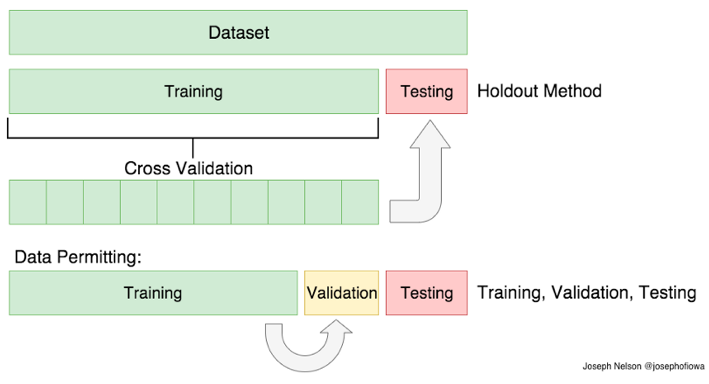
\includegraphics[width=\linewidth]{cv}
\end{center}

\begin{center}
    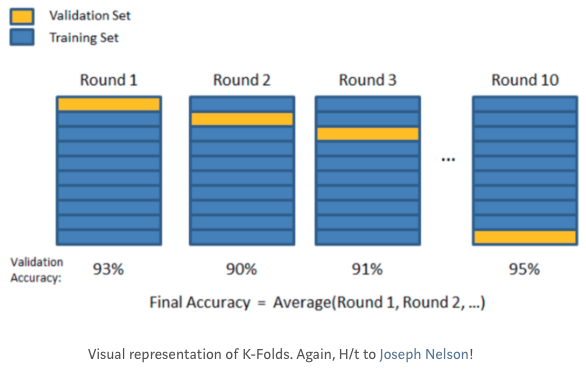
\includegraphics[width=\linewidth]{kfoldrep}
\end{center}
}

\headerbox{3. Results}{name=screen,span=2,column=1,below=introduction}{ % To reduce this block to 1 column width, remove 'span=2'

\begin{wrapfigure}{l}{0.35\textwidth}
    \vspace{10pt}
    \begin{center}
        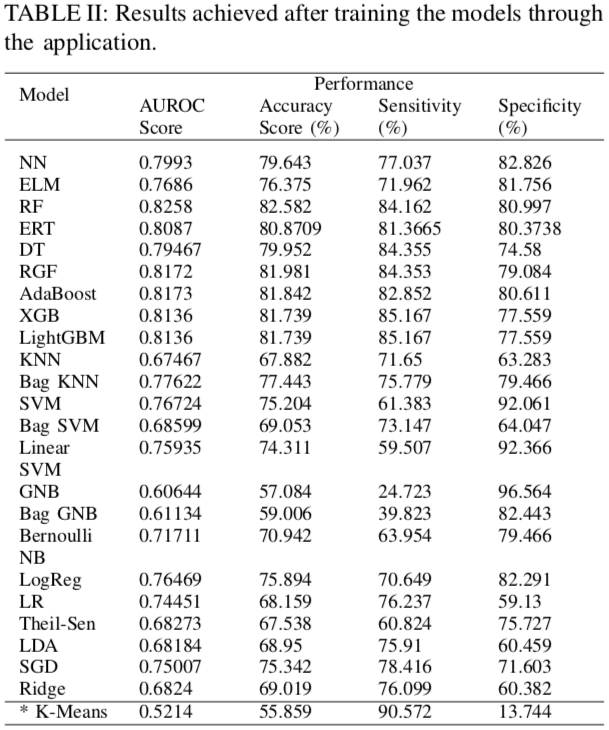
\includegraphics[width=\linewidth]{r1}
    \end{center}
    %\vspace{-145pt}
\end{wrapfigure}

At every fold during the cross-validation process, each model returns a set of predictions, which the application stores. At the end of all iterations (10 iterations, since the cross-validation method implemented, is tuned to partition the data in 10 folds), the mean for every performance metric and each executed algorithm was calculated.

\hspace{0pt}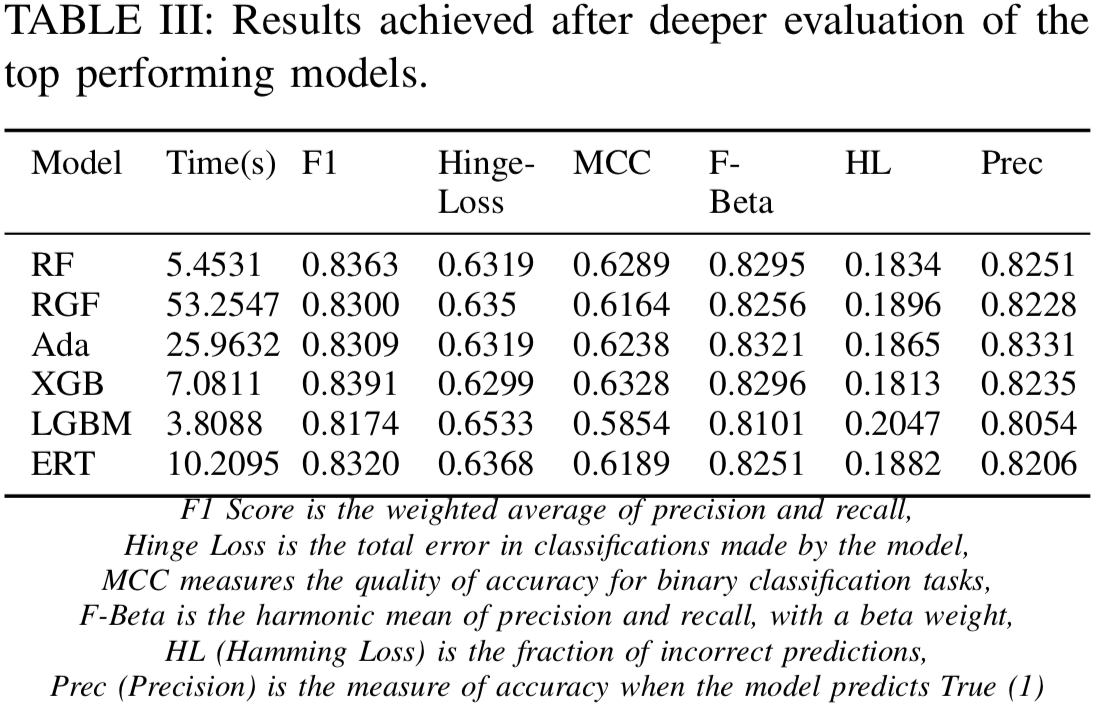
\includegraphics[width=\linewidth]{r2}

}

\headerbox{4. Discussion}{name=sea,span=2,column=1,below=screen}{ % To reduce this block to 1 column width, remove 'span=2'

Similarly to what Percy et al. \cite{percy_predicting_2016} achieved, the sequential NN model produced very close results to the RF with a mean accuracy score of 79.643\% and 82.585\% respectively. The ELM approach achieved comparable results to the NN. Sensitivity wise, the boosting methods LightGBM and XGBoost achieved the highest score out of the whole bunch as a result of 85.167\%. RF achieved the highest overall accuracy and AUROC score of 82.582\% and 0.8258 respectively. Concerning the sensitivity score, the least performing model was the GNB achieving an abysmal result of 24.72\%. The SVM model performed quite mediocre, achieving an overall AUROC and accuracy of 0.76724 and 75.204\% respectively.\\

\raggedright

Theil-Sen ranked with the set of lower performing models, achieving an overall AUROC of 0.683, with an even more inferior sensitivity score of 60.82\%. Similarly, LDA produced close AUROC results with an improved sensitivity value, still below average. Both the LogReg and LR models achieved better performance than the latter. Since LR managed a specificity value of only 59.13\%, this implies that 40.87\% samples were classified incorrectly. The K-Means clustering algorithm achieved the worst results. This technique is highly sensitive to data scaling and the range of values, which could explain the poor performance. Moreover, this algorithm also assumes that all features present are continuous, and even if transforming these variables to dummy-variables, this could negatively affect its performance.
\begin{center}
  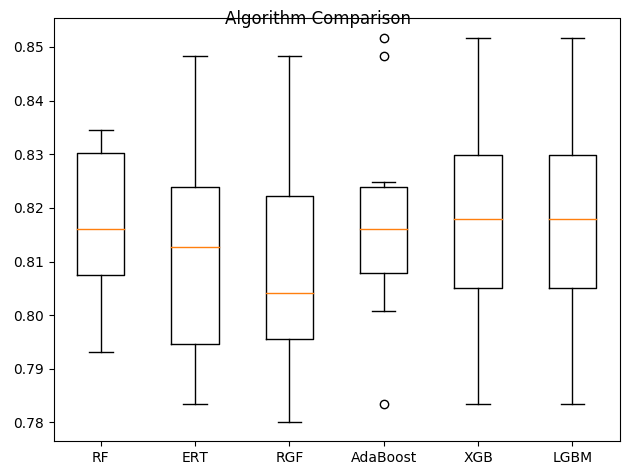
\includegraphics[width=0.35\linewidth]{deep}
\end{center}
}


\headerbox{5. Conclusions}{name=conclusion,column=1,below=sea,span=2,above=bottom}{
% DeCAF is a chemoinformatical tool that can be helpful in ligand-based drug design.
% It provides a comprehensive molecule description and a fast algorithms for comparing and aligning multiple ligands.
This research proves that Random Forests and the boosting methods LightGBM and XGBoost are amongst of the most highly effective techniques to predict and classify players as either exhibiting problematic behaviour characteristics or not.

\begin{boenumerate}\compresslist
    \item All three algorithms achieved over 80\% accuracy across all of the performance metrics calculated.
    \item These three approaches achieved the top three execution times.
    \item These three methods were the most consistent out of all the evaluated techniques.
\end{boenumerate}
% It can be also used in other [procedures], such as database screening or drug repositioning.
% DeCAF is written in Python and freely available at \textbf{\color{darkgreen}http://bitbucket.org/marta-sd/decaf}. 
}


\headerbox{6. References}{name=references,column=0,span=1,below=model,above=bottom}{


%\small % Reduce the font size in this block
\renewcommand{\section}[2]{\vskip 0.05em} % Get rid of the default "References" section title
%\nocite{*} % Insert publications even if they are not cited in the poster


\bibliographystyle{unsrt}
\bibliography{poster} % Use sample.bib as the bibliography file
}

\end{poster}

\end{document}
